\section{Drummer Overview}
\label{sec:overview}


\begin{figure}[H]
\centering
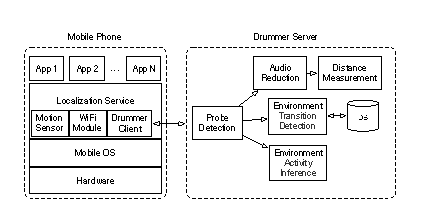
\includegraphics[width=0.45\textwidth]{./fig/arch.eps}
\caption{System Architecture of Drummer \fxnote{am I mixing arch and algorithm here?}}
\label{fig:arch}
\end{figure}


The system archtecture of Drummer is shown in figure \ref{fig:arch}. The mobile phone drummer 
client keeps minimum work and offloads data and computation to the cloud. In this paper, we assume 
network connectivity are awalys sufficient to stream audio data. Tackling with bad network conditions 
\cite{cuervo2010maui} and optimizing audio streaming \cite{farleycsense} are also important 
problems, but they are outside the scope of this paper. A drummer server maintains a TCP connection
with each client for upstream audio streaming and downstream event-based environmental information
retrieved from sound. The drumer server implements all algorithms we will discuss in next section.


\subsection{Mobile Phone Client}

The mobile phone drumer client sits in between mobile phone operating system and applications.
It provides asynchronize APIs for applications to get updates of the latest estiamted features of
current spatial environment. The current proposed and implemented features are discusses in next section.
The client initializes a TCP connection to server, keeps streaming the audio data to Drummer server, 
and receives different types of environmental features, as described next.



\subsection{Drummer Server}

Server is 